% Lab 4:
% DAQ
\chapter{Introduction to Data Acquisition and Real-Time Control}

The objectives of this laboratory session are:
\begin{itemize}
\item
    Gain familiarity with the Quanser MultiQ8 board and WinCon Software.
\item
    Understand the basic input/output (I/O) connections.
\item
    Create a WinCon application for the encoder and measure the encoder angle.
\item
    Create a WinCon application to run the motor and measure the tachometer and potentiometer signals.
\end{itemize}

\section{Pre-Lab Assignment}

Read the following introduction and skim the wiring and connection diagrams in this lab handout.
\par
Digital control of a continuous-time systems has become very popular as the price and reliability of digital computers has improved.  Digital sensors (like thermocouples in thermostats) and a computer (like an integrated circuit)  perform calculations to emulate the analog controllers (like bi-metal strips) they replace.  Very complicated control structures can be implemented easily using a digital controller, whereas an analog controller would require complex hardware.  Digital controllers are more adaptable to parameter changes than their analog counterparts.  Furthermore, analog emulation and real-time control provide advanced features such as adaptive self-tuning, multivariable control, expert systems, and the ability to communicate over a local area network.
\par
Typically, the computer replaces the cascade controller.  The measured data is converted from analog to digital form by the analog-to-digital converter (ADC).  This is accomplished by the data acquisition system (DAQ) which is the ``eyes and ears'' of the digital computer.  The computer receives and manipulates the signal in digital (binary) form, and the output is then converted to analog by the digital-to-analog converter (DAC).  This process is the ``hands and arms'' of the computer.
\par
The full scale output is usually determined by an external reference voltage.  The DAC resolution is defined as the smallest possible change in output.  For an $N$-bit converter the resolution is given by Eq.\ (\ref{eq.outputresolution}).
\begin{equation}
    \mbox{Resolution } = \frac{100}{2^N}\%
    \label{eq.outputresolution}
\end{equation}
For example, the resolution of a $10$-bit DAC is
\begin{equation*}
    \frac{100}{2^{10}} = \frac{100}{1024} = 0.09766\%
\end{equation*}
The resolution of an ADC is defined as the smallest detectible change in input, which is also given by (\ref{eq.outputresolution}).
\par
When the computer reacts to external events as they occur, it is referred to as \uline{real-time} control.  An important consideration in real-time control is the update rate.  During one controller cycle, three things must happen before the next cycle can begin:
\begin{inparaenum}[1)]
\item
    Sensors are read (ADC inputs),
\item
    The microprocessor computes updated commands, and
\item
    The commands are converted to analog signals (DAC outputs).
\end{inparaenum}
Between cycles, the commands outputs are held constant.  If the controller is updated every 0.01 seconds, the output of the controller would look like a staircase with steps 0.01 seconds wide.  As expected, the faster the dynamics of the system being controlled (pouring water versus pouring molasses), the faster the update rate must be.
\par
Modern real-time control systems use computer aided software engineering (CASE) such as MATLAB's Real-Time Workshop to automatically generate C code from a graphical control model (like Simulink).  Often the sensors or other components of the DAQ system are proprietary.  Vendors now provide Simulink blocks along with their hardware in order to ease the graphical modeling of their product.
\par
In this lab, we will focus on gaining familiarity with the MultiQ8 DACB and WinCon software.  In addition, you will explore the effects of A/D and D/A conversion that are built into the MultiQ8 board through which all the control signals pass.

\section{Laboratory Procedure}
This experiment requires four items to be connected; the parenthetical comments are what these devices will be commonly referred to hereafter:
\begin{enumerate}
\item SRV-02 Motor (plant)
\item MultiQ8 data acquisition board (DAQ board)
\item Universal power module (UPM)
\item computer (CPU)
\end{enumerate}

\subsection{Wiring Connections}
The proper connection of these elements is crucial---and particularly confounding in the tight spaces on the lab bench.  The connections are detailed in Table~\ref{tab.daqconnections} and pictured as a whole in Figure~\ref{fig.daqconnections}.

\begin{table}[bht]
\centering
\renewcommand{\arraystretch}{1.1}
\begin{tabular}{c | c | c | l}
    \textit{Order}  &   \textit{From}   &   \textit{To} & \multicolumn{1}{c}{\textit{Cable}} \\
        \hline \hline
    1   &   Plant ``motor''     &   UPM ``To Load'' &   4-DIN to 6-DIN \\
    2   &   Plant ``tach''      &   UPM ``S3''      &   6-DIN mini to 6-DIN
                                                        mini \\
    3   &   Plant potentiometer ``S1 \& S2''
                                &   UPM ``S1 \& S2''&   6-DIN mini to 6-DIN
                                                        mini \\
    4   &   DAQ ``Encoder 0''   &   Plant ``Encoder''&  5-DIN to 5-DIN \\
    5   &   DAQ ``Analog Output 1''
                                &   UPM ``From D/A''&   Phono to 5-DIN \\
    6   &   DAQ ``Analog Input 1--4''
                                &   UPM ``To A/D''  &   4xRCA to 5-DIN \\
    7   &   DAQ ``Cable 1--3''  &   CPU             &   Serial bus ribbons
\end{tabular}
\caption{\footnotesize
        Wiring connections for basic experimental setup
        \label{tab.daqconnections}
        }
\end{table}

\begin{figure}[bht]
\centering
\includegraphics[height=.9\textheight]{2590Setup}
\caption{\footnotesize
        Proper connections for the basic experimental setup.  Note the serial bus ribbons are not shown but should connect to the DAQ board as indicated.  They are size-keyed so that it is clear where they plug in.
        \label{fig.daqconnections}
        }
\end{figure}

Do not power up the amplifiers.  Make sure the LED on the DAQ board is illuminated.  If it is not, then the fuse needs replacement.  Contact the instructor.
\par
Close-up photographs of the equipment with connection details are provided in Figure~\ref{fig.equipmentcloseups}.

\begin{figure}[thb]
\centering
\subfloat[
    \footnotesize
    SRV-02 Plant.  (A) goes to UPM ``To Load.''  (B) goes to UPM ``S3.''  (C) goes to DAQ ``Encoder'' position 0.  (D) goes to UPM ``S1 \& S2.''
    ]{
    \includegraphics[width=.45\textwidth]{2594Plant}
    }
\hfill
\subfloat[
    \footnotesize
    MultiQ8 Data Acquisition (DAQ) board.  (E) goes to Plant ``Encoder.''  (P) goes to UPM ``From D/A.''  (RWYK) bundle and go to UPM ``To A/D.''
    ]{
    \includegraphics[width=.5\textwidth]{2607MultiQ}
    }
\newline
\subfloat[
    \footnotesize
    Universal power module (UPM).  (A) goes to DAQ ``Analog Outputs'' position 0.  (B) goes to Plant ``S1/S2.''  (C) goes to Plant ``Tach.''  (D) goes to Plant ``Motor.''  (E) goes to DAQ ``Analog Inputs'' positions 1 (yellow), 2 (white), 3 (red), and 4 (black).
    ]{
    \includegraphics[width=.75\textwidth]{2596UPM}
    }
\caption{\footnotesize
        Equipment connection details
        \label{fig.equipmentcloseups}
        }
\end{figure}

\clearpage
\subsection{Create the Simulink Model}
The encoder is used to provide the digital phase information.  Start MATLAB, launch Simulink, and open a new model.  From the Simulink Library, get the Encoder Input block from the Quanser Toolbox/Quanser Consulting MultiQ8 Series folder as seen in Figure~\ref{fig.multiq8libraryblock}.

\begin{figure}[bht]
\centering
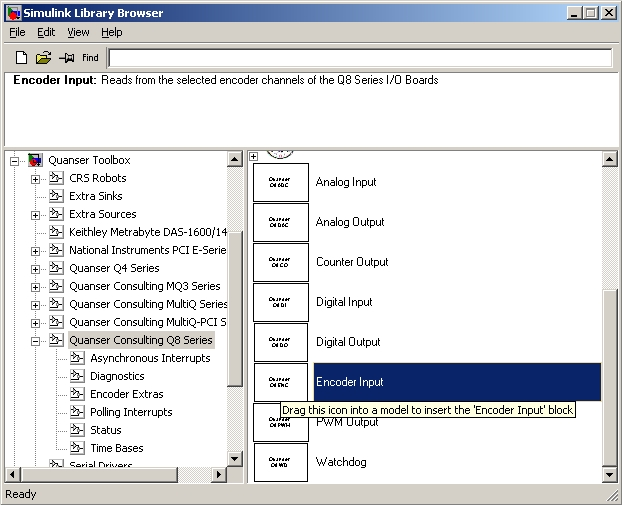
\includegraphics[width=.65\textwidth]{QuanserToolboxScreenshot}
\caption{ \footnotesize
        Simulink library including the proprietary Quanser Q8 toolbox
        \label{fig.multiq8libraryblock}
        }
\end{figure}

Draw a Simulink diagram as shown in Figure~\ref{fig.encodermeasure}.  The encoder input is connected to Encoder~0 on the MultiQ wiring diagram.  Double-click on the Encoder input block to open its dialog box and set the ``Channel to Use'' to 0.  Save the model.

\begin{figure}[bht]
\centering
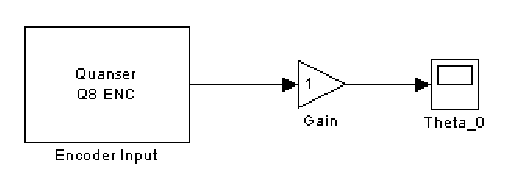
\includegraphics[width=.5\textwidth]{encoderonly}
\caption{\footnotesize
        Simulink diagram for encoder experiment
        \label{fig.encodermeasure}
        }
\end{figure}

There are a few tips for drawing Simulink models.  It is often easiest to place all the blocks in rough positions first.  To connect blocks, try this: Click on the origin block, hold the \textit{Control} key, and click on the destination block.  This can be repeated until all blocks are appropriately connected.
\par
Also, it is sometimes helpful to rename blocks so that we can recognize them later.  For example, Simulink models often have many Gain blocks.  Instead of having them named Gain, Gain1, Gain2, and so on, single-click on the name in the model and rename them with something more descriptive.

\subsection{Compiling the Model}
If you choose to use a mobile machine to run the experiments, read the following.  If not, please skip the boxed material.
\par \noindent
\begin{center} \setlength{\fboxrule}{0.5pt}
\fbox{\parbox{.9\textwidth}{\vspace{-6pt} \begin{flushleft}
\textbf{Optional Instructions for Remote Connections} \end{flushleft}
\parbox{.9\textwidth}{ \small
Before you run any real-time code, you need to launch the WinCon server and connect to the client PC where the experiment is going to run.  Ensure that WinCon Client is running on the PC you want to connect to.  Start the WinCon server on your laptop and then use Client\textrightarrow Connect as shown in Figure~\ref{fig.clientconnect}.  In the dialog box, enter the proper client workstation IP address (The station IP addresses are s312-1 to s312-10).
}
}
}
\end{center}

\begin{figure}[bht]
\centering
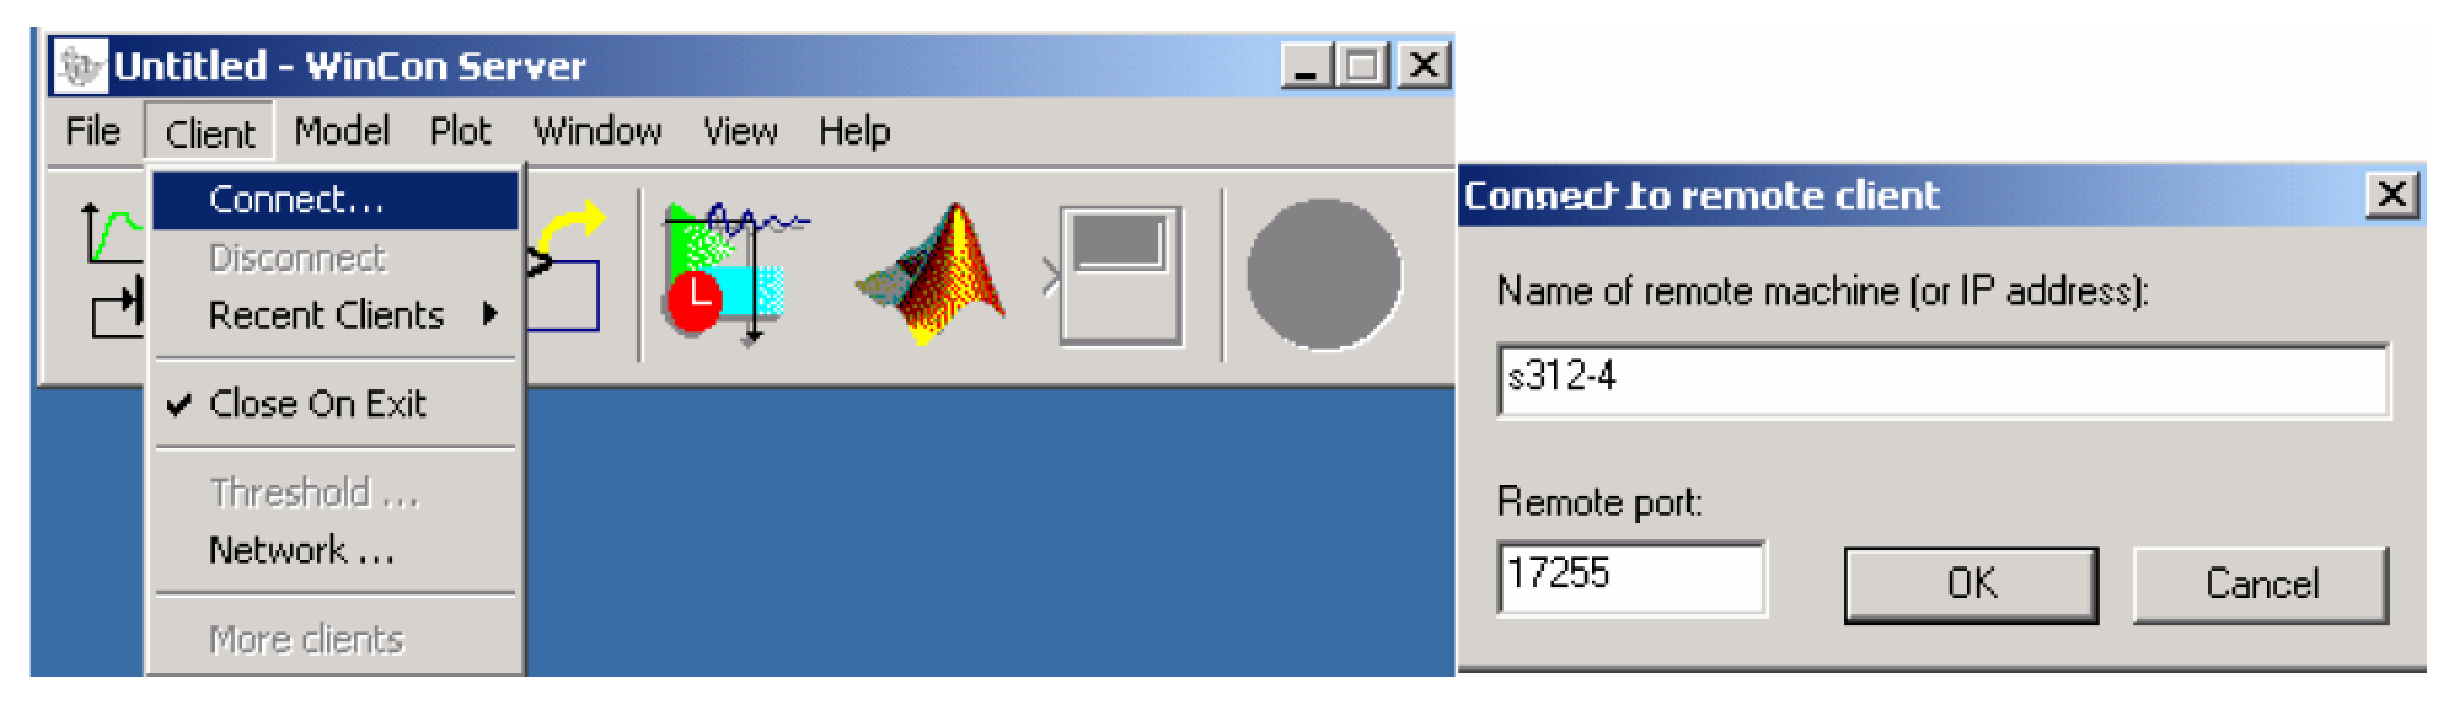
\includegraphics[width=.6\textwidth]{clientconnect}
\caption{ \footnotesize
        Remote connection to the client that is running the experiment
        \label{fig.clientconnect}
        }
\end{figure}

In order to run the simulation in real-time, you must first build the code for it.  This is done using the WinCon\textrightarrow Build option seen in the diagram in Figure~\ref{fig.winconbuild}.  However, there are several simulation parameters that need to be set before building the model.

\begin{figure}[bht]
\centering
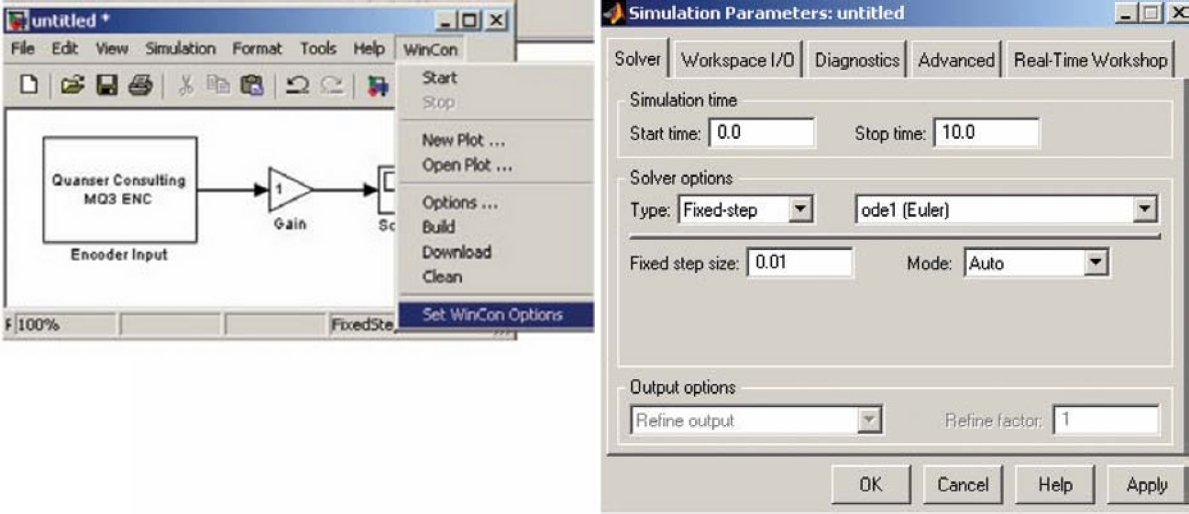
\includegraphics[width=.75\textwidth]{winconbuild}
\caption{ \footnotesize
        WinCon dropdown menu in Simulink.  Simulation parameters are set as shown in this menu under ``Set WinCon Options.''  When ready, the model is built with WinCon\textrightarrow Build.
        \label{fig.winconbuild}
        }
\end{figure}

Select WinCon\textrightarrow Options to open the Simulation Parameters dialog box.  Choose the Solver tab and set the sampling rate on the controller to a fixed step size of 0.01 seconds.  Also, select ``ode4 (Runge-Kutta)'' as the integration method.  In the Simulation dropdown menu, set the model to ``External.''
\par
Now click WinCon\textrightarrow Build.  This will generate the code and compile it.  It may take a while depending on the machine you are working on.  When the compile is done, the code will download to the WinCon Client.  You can now use the WinCon Server to start and stop real-time code.  These two windows are shown in Figure~\ref{fig.clientserver}.  If it is not open already, open the WinCon Server; we will need it in the next section.

\begin{figure}[hbt]
\centering
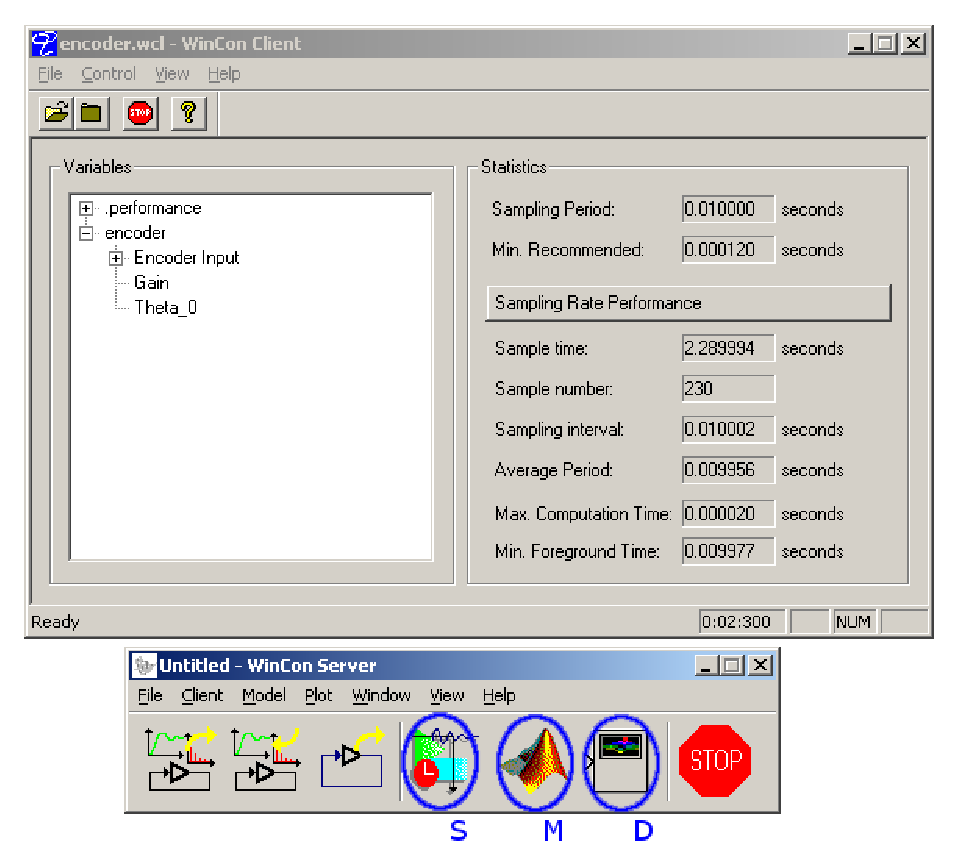
\includegraphics[width=.6\textwidth]{clientserver}
\caption{ \footnotesize
        WinCon Client (above) and Server (below).  The (S) button brings up the pertinent Simulink model, (M) brings up the MATLAB window, and (D) opens the WinCon Display Dialog.
        \label{fig.clientserver}
        }
\end{figure}

\subsection{Encoder Signal}
Now we are ready to see the real-time code in action.  To visualize the data, WinCon offers the Display button next to the Start/Stop button.  This links to all of the output displays we built into our Simulink model.  For this experiment, we should have a trace available called \textit{Theta\_0}.  Open this trace and start the experiment.
\par
With WinCon running, rotate the gears of the plant (by hand) and observe the real-time trace.  The default time span is five seconds.  To increase this, go to Update\textrightarrow Buffer and change to the desired amount.  You can, of course, at any time stop the experiment by clicking on the big red Stop button in the WinCon Server.
\par
In a blank trace window, rotate the big (central) gear 45\textdegree\ counterclockwise (ccw), then back 90\textdegree\ clockwise (cw), and then back to the starting position.  Stop the experiment.  There is no need to be terribly exact, we are primarily concerned with the sign of the encoder for this motion.
\par
Hopefully your trace will look something like Figure~\ref{fig.angletrace}.  If your counterclockwise motion produced negative data points, you will need to change the gain block in your Simulink diagram from $+1$ to $-1$.  It is important for this experiment and subsequent ones that counterclockwise motion have a positive sign and the opposite for clockwise motion!

\begin{figure}[bht]
\centering
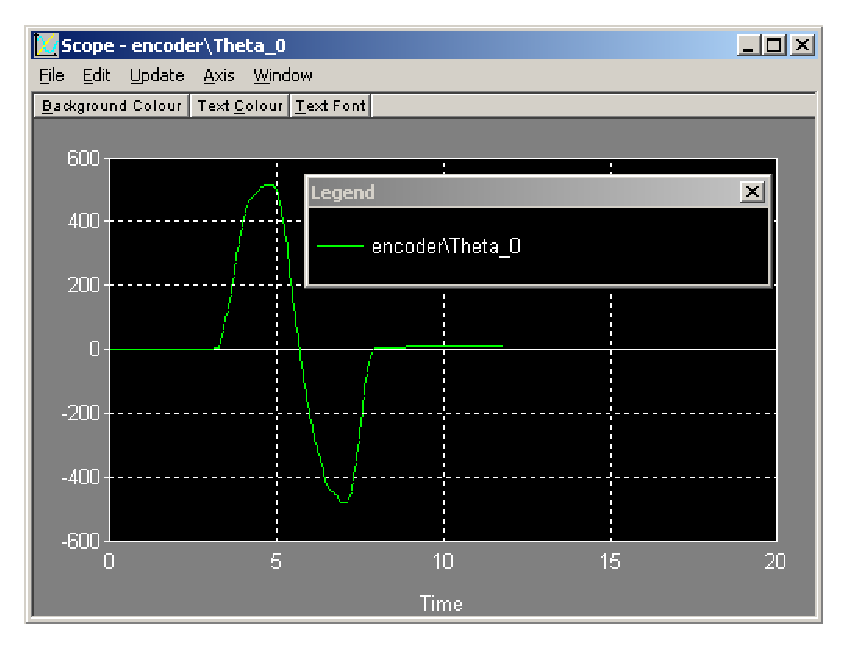
\includegraphics[width=.6\textwidth]{angletrace}
\caption{\footnotesize
        Sample trace of the encoder output.  Counterclockwise motion corresponds to positive data, so the Simulink gain block is correctly configured.
        \label{fig.angletrace}
        }
\end{figure}

To add a legend to the trace, use the Window dropdown menu.
\par
Here it is important to note that we can import the data seen by WinCon to MATLAB.  In the trace window, the File\textrightarrow Save menu allows us to export the data points as an m-file, a mat-file, or directly to the MATLAB workspace as variables.
\par
With MATLAB, observe the numerical data recorded for the $\pm$45\textdegree\  run.  In particular, note the following:
\begin{enumerate}
\item
    Does the data start and end at zero?  Why is this?
\item
    What are the maximum and minimum data points?  Why are they not $+45$ and $-45$?
\item
    How could you calculate the speed at which you turned the gears from this data?  What would the units be?
\end{enumerate}

We will focus on Item 2.  The others are appropriate to be addressed in the lab report.
\par
As you noted, the encoder did not record 45\textdegree---or anything close---when you turned the gears by about that amount.  This is because the encoder uses proprietary units called \uline{counts}.  The encoder measures 1024 counts per revolution in quadrature.  Thus a rotation of 360\textdegree\  results in $1024\times4 = 4096$ counts.  This means that the resolution of the encoder is $360/4096 = 0.087890625$\textdegree.
\par
In order to have future data in degrees, change the gain block in the Simulink model (Fig.\ \ref{fig.encodermeasure}) to $360/4096$ with the appropriate sign.

\subsection{Sensor Calibration}
Now that we have some experience with drawing a Simulink model, building the real-time code, and interfacing with WinCon, we are ready to observe and calibrate the equipment.  The motor on the plant is driven by an amplifier that can deliver the desired power to it.  In order to drive a voltage to the motor, we need to output the desired voltage to the correct D/A channel.  From the wiring we performed (see Table~\ref{tab.daqconnections} and Fig.\ \ref{fig.daqconnections}), we know that DAC Channel 1 drives the UPM, which in turn drives the motor.
\par
Click File\textrightarrow New in WinCon---do not save anything.  Start a fresh Simulink diagram (see Figure~\ref{fig.calibratemodel}).  Use the same simulation parameters from the encoder model, except change the fixed step size to 0.001~seconds.  Connect a constant block via a gain to the Quanser Analog Output block.  This will output a constant voltage to the channel specified in the output block's parameters (double-click).
\par

\begin{figure}[bht]
\centering
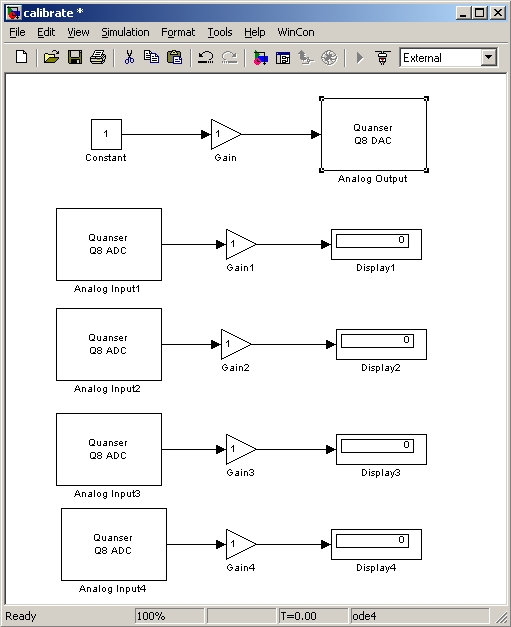
\includegraphics[width=.6\textwidth]{calibratemodel}
\caption{\footnotesize
        Simulink model for sensor calibration
        \label{fig.calibratemodel}
        }
\end{figure}

Next, add four analog input blocks (one for each of the RCA plugs on the DAQ board).  Connect them all to display blocks via unity gains.  Be sure to set their Channels to 1--4.  Now we are ready to build the code.
\par
\noindent\parbox{\textwidth}{
\mbox{\Large \textbf{Important}:}\\[3pt]
\indent \large Whenever you run an experiment that sends power to the motor, one team member must be assigned to operate the amplifier power switch.  Located on the back of the UPM, the ``kill switch'' is the only fail-safe method to cut power to the plant.\\[3pt]
\indent We do not know the internal gains associated with the plant and power module mechanisms.  How do we know that the constant ``1'' block will not overload the motor?  Mistakes \textit{do} happen, so to protect yourself, your teammates, and the equipment, always have someone ready to cut power in the event of an accident.
}

\vspace{6pt}

\par
In the WinCon Server, create four displays for the four sensor readings.  With a teammate on the kill switch, start the experiment.  Note that we have sent a positive constant voltage to the motor.  If the central gear rotates counterclockwise, then this is correct.  If it does not, change its gain to $-1$.
\par
Upon observing the four displays, you should see
\begin{itemize}
\item
    Two that hover around zero,
\item
    One that will remain relatively constant at a value other than zero, and
\item
    One that will revolve widely about zero.
\end{itemize}
From this, we know that the two channels that display zero data are not used.  We do not need to include them.  Further, the constant display is the tachometer; the revolving one corresponds to the potentiometer.
\par
Using a stopwatch, approximate the rotational speed of the central gear in revolutions per minute (rpm).  Using this measurement, change the gain block to accurately reflect the revolutions per minute (with the appropriate sign) of the system.
\par
Export the data from the potentiometer to MATLAB.  Find its minimum and maximum values.  From these, determine the calibration factor needed for the potentiometer to display in degrees.  Place this value in the potentiometer's gain block.  Also, add a scope on the potentiometer's output.
\par
After all this, your Simulink diagram should look something like Figure~\ref{fig.finalcalibrationmodel}.

\begin{figure}[bht]
\centering
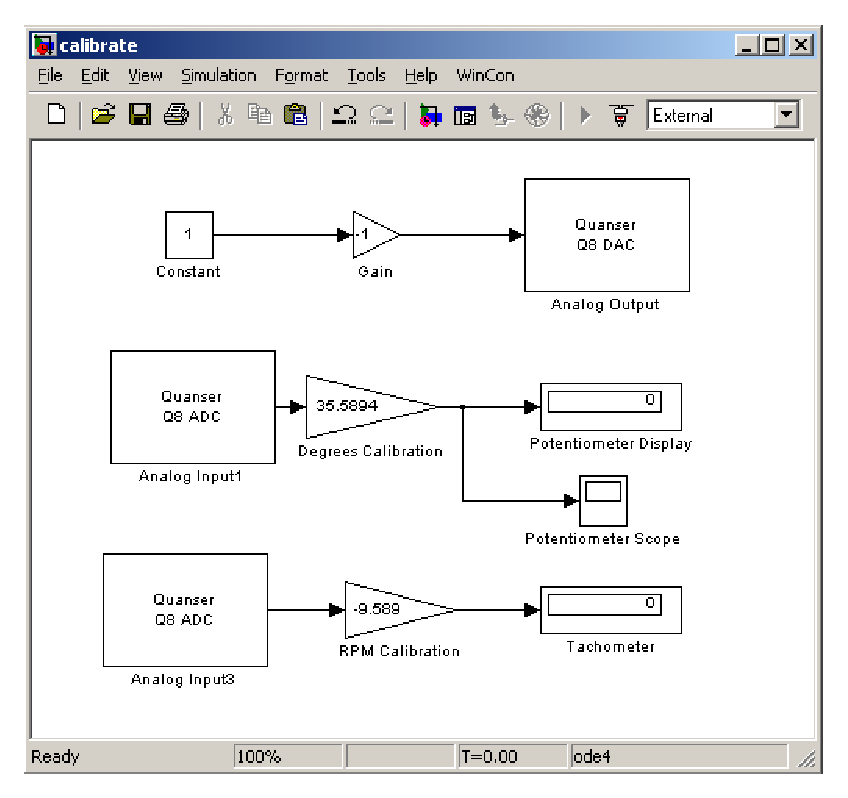
\includegraphics[width=.6\textwidth]{finalcalibrationmodel}
\caption{\footnotesize
        Example Simulink diagram with motor voltage sign inversion, tachometer calibration gain, and potentiometer calibration gain implemented.
        \label{fig.finalcalibrationmodel}
        }
\end{figure}

\par
For those interested, the potentiometer is a single-turn 10~k\textohm\ sensor with no physical stops.  Its electrical range is 352\textdegree.  The potentiometer generates an analog signal proportional to the angle of rotation.  The difference between a potentiometer and an encoder is that the encoder can measure several turns continuously while the potentiometer can only measure one full turn and then roll over.  Note that the potentiometer is an absolute position device while the encoder is a relative position device.  You can adjust the potentiometer shaft rotation relative to the gear such that the zero measurement is always at a desired angle.
\par
Create a well-labeled MATLAB plot of the calibrated potentiometer data over several periods of rotation.
